\documentclass[12pt]{elegantbook}

\definecolor{LightGray}{gray}{0.9}
\newcommand{\CN}{BIOS 7300\\[0.5cm] Survival Data Analysis}
\newcommand{\Ti}{Homework 3}
\newcommand{\Pf}{Dr. Tang}
\newcommand{\FN}{Zehao}
\newcommand{\LN}{Wang}
\usepackage[fontsize=14pt]{fontsize}

\usepackage{minted}

\usepackage{enumitem}
\renewcommand{\chaptername}{Homework}
\begin{document}
\begin{titlepage}
    \begin{center}    
    
\includegraphics[width=0.6\textwidth]{Tulane.png}\\[1cm]    
    
    \textsc{\Huge \CN}\\[0.5cm]
    \textsc{\large \Pf}\\[1.0cm]
    
    \textsc{\LARGE \Ti}\\[0.5cm]
    \textsc{\large \LN, \FN}\\
    {Master student in Statistics of Math Dept.}
    
    % Author and supervisor
    
    \vfill
    
    % Bottom of the page
    {\Large \emph{\today}}
    
    \end{center}
\end{titlepage}

\thispagestyle{empty}
\tableofcontents
\setcounter{chapter}{2}
\chapter{}

    
    \begin{exercise*}[1]
        The table on the next page contains the KM estimate of the survival function $(S)$ and its point-wise $95\%$ confidence intervals (LCL=lower limit and UCL=upper limit), where $c$ is the censoring indicator ($0$ means not censored, and $1$ means censored). Based on the table, find the following quantities. If any of these quantities are undefined, explain. 
        \begin{enumerate}[(a)]
            \item The median survival time, and the $95\%$ confidence interval for the median.
            \item The first and third quartiles, and the $95\%$ confidence intervals for these quartiles.
            \item The SIQR. 
        \end{enumerate}
        \begin{figure}[H]
            \centering
            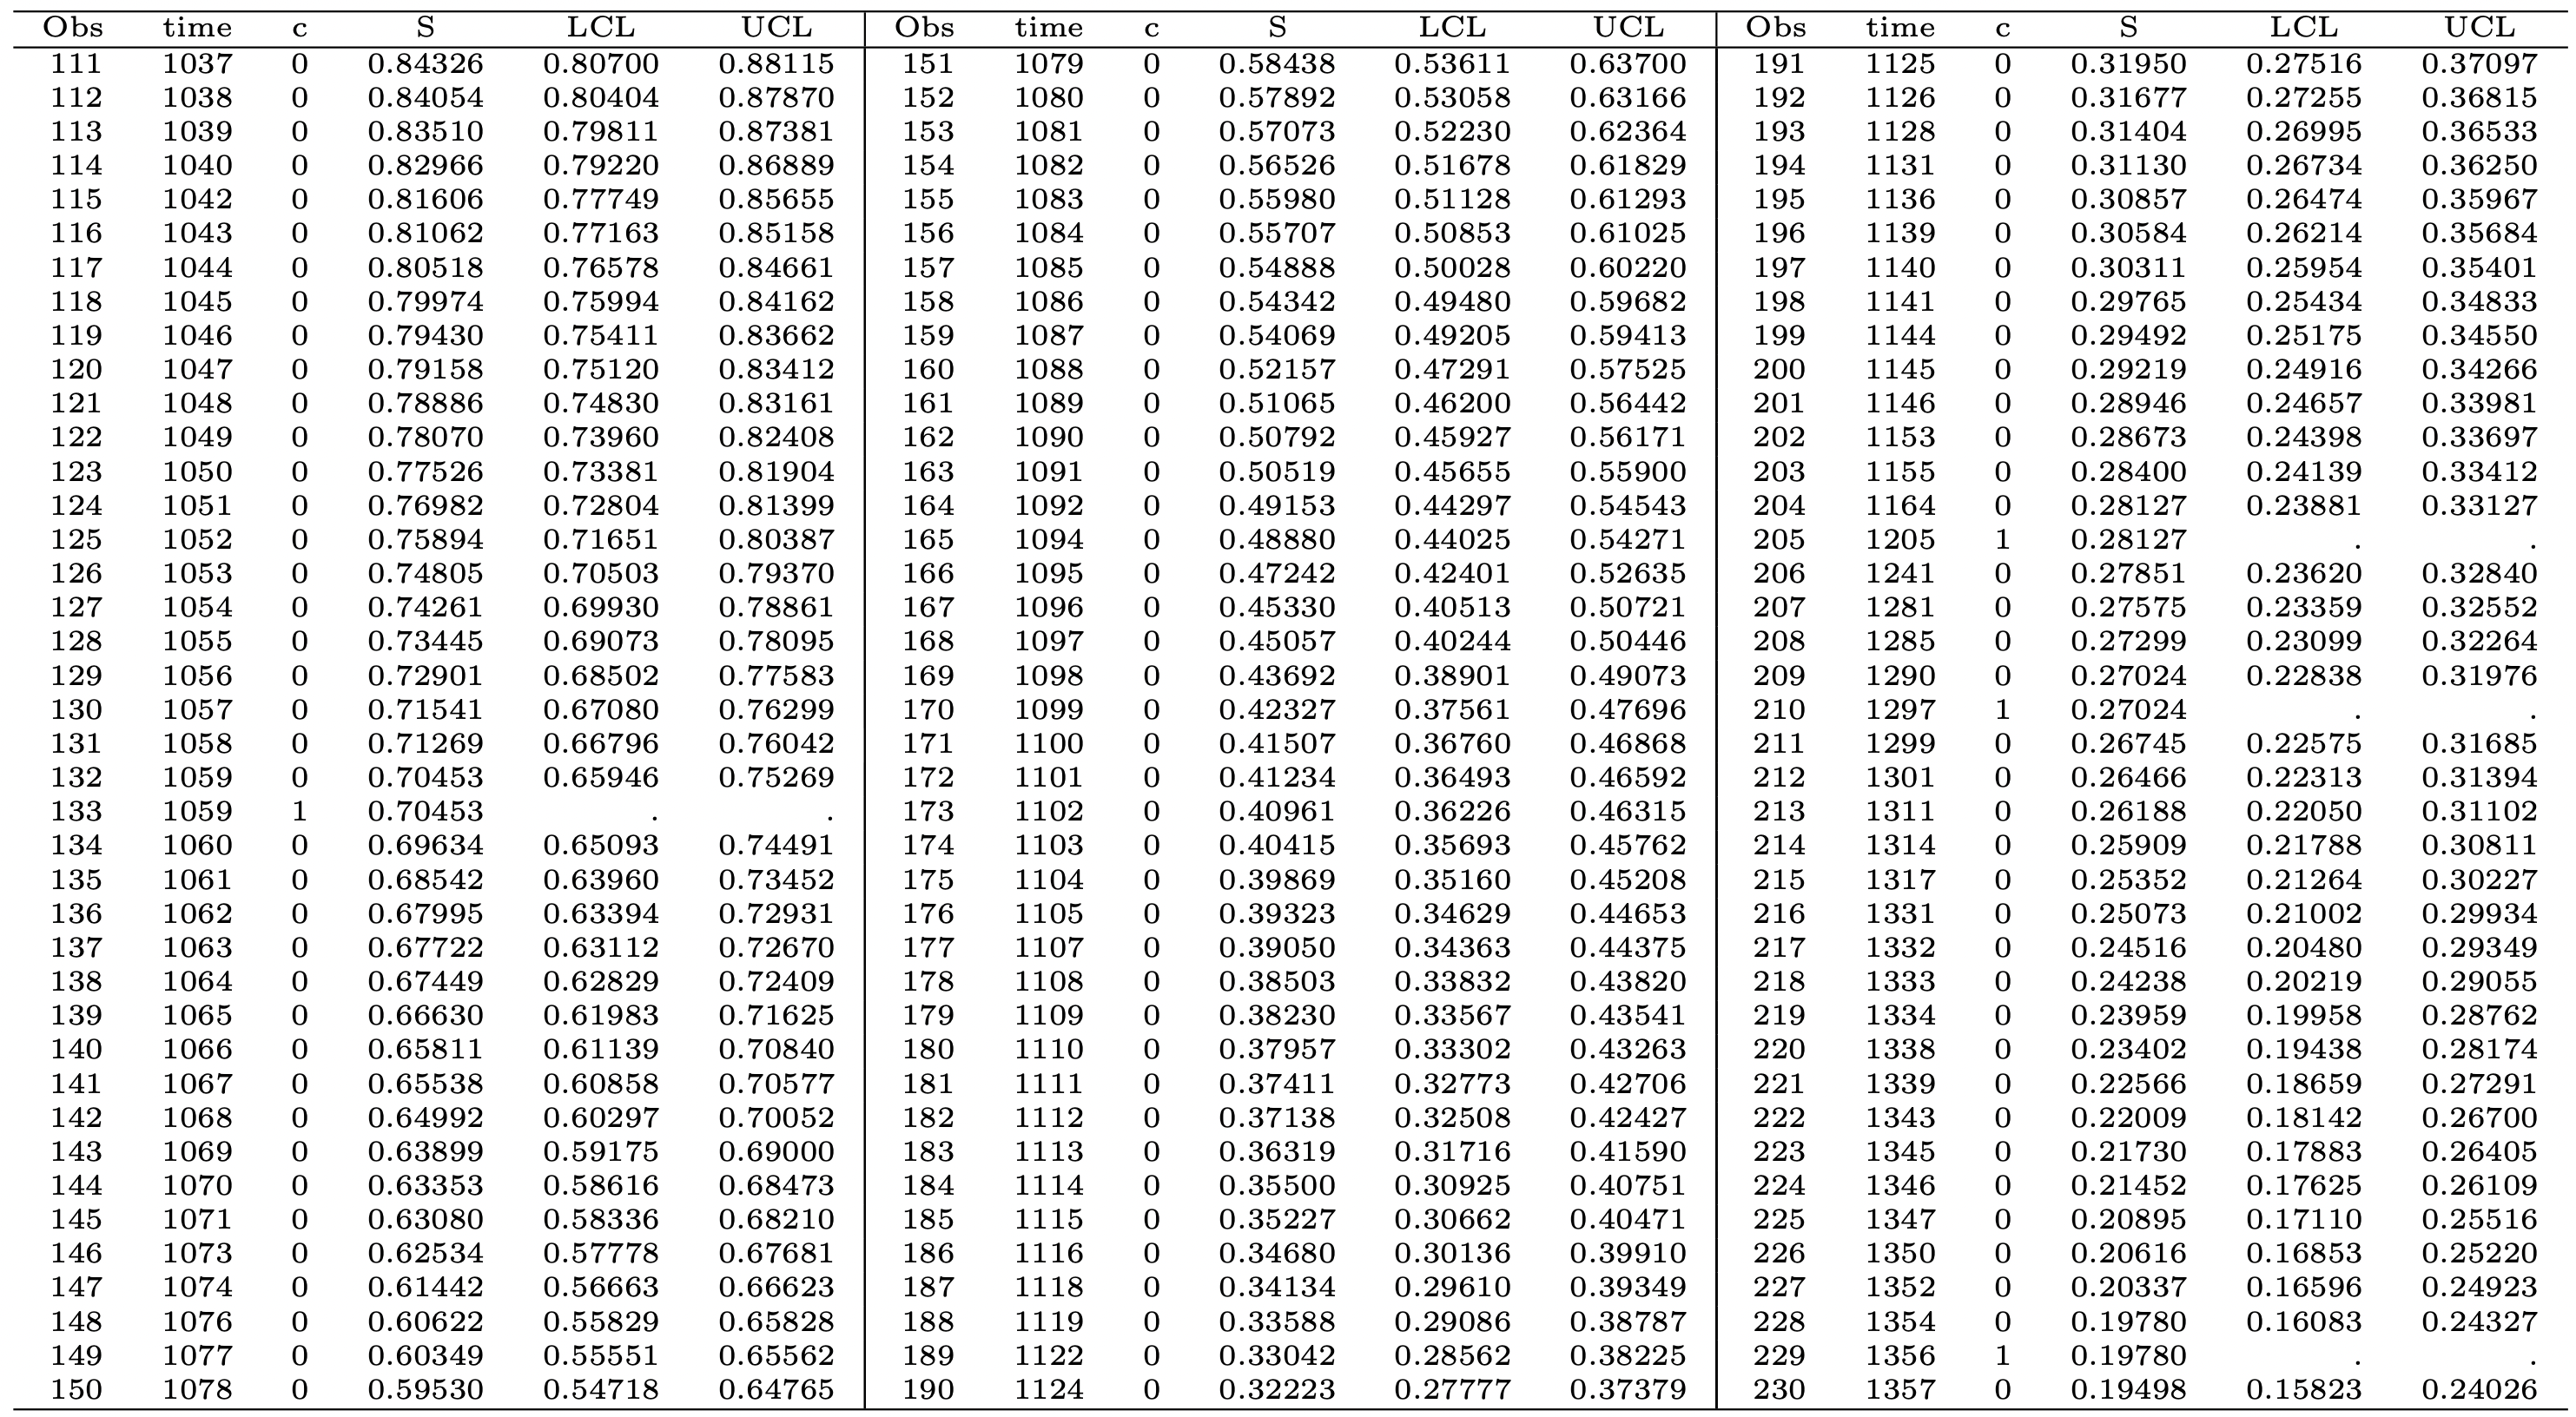
\includegraphics[width=\textwidth]{HW1_4.png}
        \end{figure}
    \end{exercise*}
    \begin{solution}
        \begin{enumerate}[(a)]
            \item Median survival time is: 
            \[t=\min\{t:S(t)\leq0.5\}=1092. \] 
            With this same condition on LCL and UCL, we can get the $95\%$ confidence interval for the median is \[[t_{LCL},t_{UCL}]=[1086,1098]. \]
            \item First quartile is: $t=\min\{t:S(t)\leq0.75\}=1053$. And the $95\%$ confidence interval for the first quartile is $[t_{LCL},t_{UCL}]=[1053,1060]$. 
            
            Third quartile is: $t=\min\{t:S(t)\leq0.25\}=1332$. The $95\%$ confidence interval for the third quartile is $[t_{LCL},t_{UCL}]=[1145,1352]$. 
            \item \[SIQR=(t_{0.75}-t_{0.25})/2=139.5. \]
        \end{enumerate}
    \end{solution}


    \begin{exercise*}[2]
        The survival times used in the last homework assignment actually came from two treatment groups, one with patients treated with a new treatment and the other with patients treated as usual (TAU). The survival times for the two groups are:

        New: 3, 3*, 4*, 5, 10, 12, 20, 20, 21, 24, 48, 48*
        
        TAU: 3, 5*, 18, 20, 22, 22*, 23, 48*

        (right-censored times are denoted by a *)

        \noindent Compute by hand the log-rank and generalized Wilcoxon tests for the equality of the two survivorship functions for the two groups. What conclusions can you make about the equality of the two survivorship functions? Which assumptions do you need for the computation? 
    \end{exercise*}

    \begin{exercise*}[3]
        Information of survival times for liver transplant study is recorded in the file ``Time to death while waiting for a liver transplant.dat" in the data sets folder on canvas. Separate the patients into three age groups: age $\leq50$, $51-60$, and $> 60$. 
        \begin{enumerate}[(a)]
            \item Compare the survival times across the three age groups using log ranks and Wilcoxon tests, ignoring the order of the age groups. 
            \item We expect there is a trend in the survival time associated with the age, and apply a trend test. Summarize your results.
            \item Compare parts (a) and (b). 
        \end{enumerate}
    \end{exercise*}

    \begin{exercise*}[4]
        Using the data set in the last problem. 
        \begin{enumerate}[(a)]
            \item Test if there are differences in survival times between males and females, controlling for age group (stratified by age group). 
            \item Test if there are differences in survival times across age groups (ignoring the order of the age groups), controlling for gender (stratified by gender).
        \end{enumerate}
    \end{exercise*}
\end{document}